\documentclass{beamer}
\usepackage{pgfplots}
\usetheme{progressbar}
 
 
\usecolortheme{crane}
 
 
\setbeamercolor{frametitle}{fg=brown}
 
 
\title{Analizador L\'exico}
\subtitle{Proyecto 1}
\author{Ariana Berm\'udez,Ximena Bola\~nos, Dylan Rodr\'iguez}
\institute{Instituto Tecnol\'ogico de Costa Rica}
\date{\today}
\begin{document}
\begin{frame}
 \titlepage 
 \end{frame}\begin{frame}
 \frametitle{An\'alisis L\'exico}
 Se hizo un analizador l\'exico con la ayuda de la herramienta Flex, para el lenguaje C y que corre en C, este analizador encuentra los tokens y busca su tipo, e incrementa el contador de ese tipo para luego generar histogramas y gr\'aficos de pastel. Estos gr\'aficos son mostrados en una presentaci\'on de beamer, que ser\'a tambi\'en la salida del Scanner. En la presentaci\'on se definieron los \colorbox{red}{errores} con un subrayado rojo,y para los token se defini\'o:\begin{itemize} \item magenta para los \textcolor{magenta} {KEYWORD}  \item rojo para los \textcolor{red}{INTEGER} \item verde para los \textcolor{green} {IDENTIFIER} \item morado para los \textcolor{purple}{CONSTANT} \item azul para los \textcolor{blue} {OPERATOR} \item naranja para los \textcolor{orange} {PUNTUACTOR} \item rosado para los \textcolor{pink} {LITERAL} \end{itemize} \end{frame}\begin{frame}
 \frametitle{FLEX}
 Herramienta utilizada para realizar esc\'aneres. Este toma los valores de entrada y genera los tokens correspondientes.Seg\'un la necesidad del programador. \\ Este genera un c\'odigo fuente en C que se va a nombrar lex.yy.c en el cual se genera una funci\'on yylex() la cu\'al se encarga de analizar el c\'odigo fuente. Busca la librer\'ia –lfl después de ser compilado y se enlaza con ella, para dar como resultado un ejecutable. \\ 
 El fichero de entrada de flex tiene 3 secciones, y tiene que verse como:\\ 
 \textcolor{blue}{definiciones \\ \%\% \\ reglas \\ \%\% \\ c\'odigo de usuario} \\ 
\end{frame}
\begin{frame}
Las definiciones contienen las declaraciones de nombres, y condiciones de arranque. Un ejemplo de nuestro programa es: \newline 
\textcolor{red}{[a-zA-Z][\_a-zA-Z0-9]*   return IDENTIFIER; \newline [0-9][0-9]*    return INTEGER;} \newline 
Luego de definir estos campos se procede a explicar como funciona flex, el flex asocia las entradas, \textbf{?`pero c\'omo lo hace?}\newline 
El esc\'aner analiza poco a poco las cadenas hasta que concuerden con alg\'un patr\'on propuesto por el programador. Si se puede emparejar m\'as de una forma entonces tiene prioridad quien pueda asociar m\'as texto y si en ese caso tambi\'en son iguales entonces se elige por medio de quien est\'e antes en el fichero de entrada.\newline 
El token tendr\'a asociado el puntero a caracter global \textbf{yytext}, y la longitud en la variable global entera \textbf{yyleng}. Si no hay forma de asociarlo, se usa la regla por defecto. \newline 
\end{frame}
\begin{frame}
\frametitle{FLEX - continuaci\'on} 
\textbf{Acciones} \newline 
Todo patr\'on tiene una acci\'on asociada. Existen varias acciones, por ejemplo: si se pone \newline 
\begin{table}[]
\centering
\caption{Acciones}
\label{Acciones}
\begin{tabular}{lllll}
\cline{1-2}
\multicolumn{1}{|l|}{\%\% "texto"} & \multicolumn{1}{l|}{\begin{tabular}[c]{@{}l@{}}Har\'a que se borren todas sus aparciones\\ en la entrada.\end{tabular}}                                    &  &  &  \\ \cline{1-2}
\multicolumn{1}{|l|}{\{}           & \multicolumn{1}{l|}{\begin{tabular}[c]{@{}l@{}}Tomar\'a todo eso como parte de la acci\'on hasta \\ que encuentre la llave que lo cierra, \}\end{tabular}} &  &  &  \\ \cline{1-2}
\multicolumn{1}{|l|}{-}            & \multicolumn{1}{l|}{\begin{tabular}[c]{@{}l@{}}Hace que la acci\'on actual aplique tambi\'en\\ para la siguiente.\end{tabular}}                            &  &  &  \\ \cline{1-2}
&                                                                                                                                                            &  &  & 
\end{tabular}
\end{table}


\end{frame}
\begin{frame}
\frametitle{FLEX - continuaci\'on} 
\textbf{Acciones} \newline 
El yylex() es una funci\'on que procesa tokens desde donde lo dejaron la \'ultima vez. Directivas especiales que se pueden incluir dentro de una acci\'on \newline 
Las acciones puede modificar los yytext exepto su largo, para ello se le puede agregar un \%array y as\'i modificar totalmente la variable yytext, que es donde se guarda el valor del token actual.\\Directivas especiales:\begin{itemize} \item ECHO: copia yytext a la salida del esc\'aner  \item BEGIN: pone al esc\'aner en la codici\'on de arranque correspondiente. \item REJECT: ordena a proceder con al "segunda mejor regla." \item yymore(): despues de emparejar una regla el valor de yytext actual debe se reemplazado por el siguiente.\end{itemize}\end{frame}
\begin{frame}
\frametitle{C\'odigo Analizado}
\textcolor{green}{holaFuncion} \textcolor{orange}{(} \textcolor{orange}{)} \textcolor{orange}{\{} \\ 
 \textcolor{magenta}{int} \textcolor{green}{a} \textcolor{blue}{=} \textcolor{red}{10} \textcolor{blue}{+} \textcolor{red}{3} \textcolor{orange}{;} \\ 
 \textcolor{magenta}{int} \textcolor{green}{b} \textcolor{blue}{=} \textcolor{red}{10} \textcolor{blue}{+} \textcolor{red}{3} \textcolor{orange}{;} \\ 
 \textcolor{green}{printf} \textcolor{orange}{(} \textcolor{pink}{"Hello, its me"} \textcolor{orange}{)} \textcolor{orange}{;} \\ 
 \textcolor{magenta}{return} \textcolor{green}{true} \textcolor{orange}{;} \\ 
 \textcolor{orange}{\}} \\ 
 \textcolor{magenta}{int} \textcolor{green}{funcion} \textcolor{orange}{(} \textcolor{orange}{)} \textcolor{orange}{\{} \\ 
 \textcolor{green}{printf} \textcolor{orange}{(} \textcolor{pink}{"Esto es una funci����������������n"} \textcolor{orange}{)} \textcolor{orange}{;} \\ 
 \textcolor{magenta}{return} \textcolor{red}{0} \textcolor{orange}{;} \\ 
 \end{frame}
\begin{frame}
\frametitle{C\'odigo Analizado}
\textcolor{purple}{//"hola" } \\ 
 \textcolor{purple}{//adios oidhofhofaushoi @@ \& \textbackslash n \$ } \\ 
 \colorbox{red}{\$}\textcolor{magenta}{int} \colorbox{red}{2funcionPruebaSegunda}\textcolor{orange}{(} \textcolor{orange}{)} \textcolor{orange}{\{} \\ 
 \textcolor{purple}{/*printf("Prueba\#\&\textbackslash n")\;
	int t = c\;\#
	t++\;*/} \\ 
 \textcolor{purple}{//\#} \\ 
 \colorbox{red}{\#}\textcolor{orange}{\}} \\ 
 \textcolor{red}{40} \textcolor{blue}{+} \textcolor{green}{ERROR} \colorbox{red}{\#}\textcolor{white}{} \end{frame}
\begin{frame}
\frametitle{Histograma}
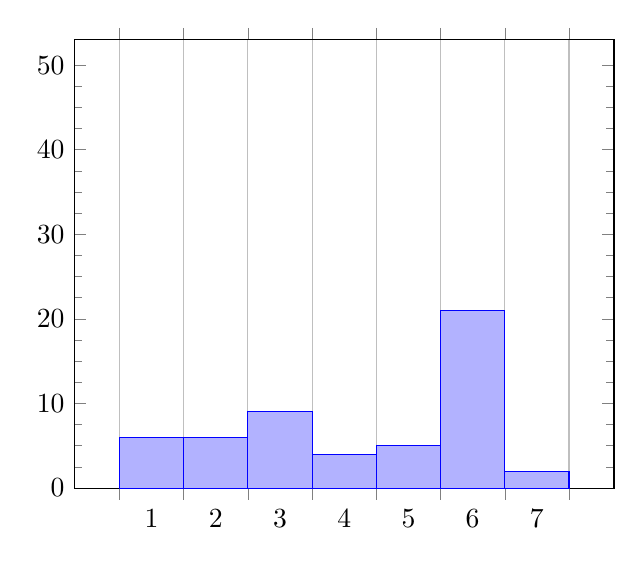
\begin{tikzpicture}
\begin{axis}[ybar interval, ymax=53, ymin=0, minor y tick num = 3]
\addplot coordinates { (1 , 6) (2 , 6) (3 , 9) (4 , 4) (5 , 5) (6 , 21) (7 , 2)  (8, 0) }; 
\end{axis}
\end{tikzpicture}
\end{frame}
\begin{frame}
\frametitle{Histograma tipo Pastel}
\def\angle{0}
\def\radius{2.5}
\def\cyclelist{{"magenta","red","green","purple","blue","orange", "pink"}}
\newcount\cyclecount \cyclecount=1
\newcount\ind \ind=3
\begin{tikzpicture}[nodes = {font=\sffamily}]
\foreach \percent/\name in {
11.32/KEYWORD,
11.32/INTEGER,
16.98/IDENTIFIER,
7.55/CONSTANT,
9.43/OPERATOR,
39.62/PUNTUACTOR,
3.77/LITERAL
 } {
\ifx\percent\empty\else
\global\advance\cyclecount by 1
\global\advance\ind by 1
\ifnum3<\cyclecount
\global\cyclecount=0
\global\ind=0
\fi
\pgfmathparse{\cyclelist[\the\ind]}
\edef\color{\pgfmathresult}
\draw[fill={\color!50},draw={\color}] (0,0) -- (\angle:\radius)
arc (\angle:\angle+\percent*3.6:\radius) -- cycle;
\node at (\angle+0.5*\percent*3.6:0.7*\radius) {\percent\,\%};
\node[pin=\angle+0.5*\percent*3.6:\name]
at (\angle+0.5*\percent*3.6:\radius) {};
\pgfmathparse{\angle+\percent*3.6}
\xdef\angle{\pgfmathresult} % and store in \angle
\fi
};
\end{tikzpicture}

\end{frame}
\end{document}
